\documentclass{article}
\usepackage[utf8]{inputenc}
\usepackage{graphicx}

\title{Report Machine Learning Second Assignment}
\author{Stefano Branchi [207523] \\ stefano.branchi@studenti.unitn.it \\\\ University of Trento}
\date{}

\begin{document}

\maketitle
\begin{abstract}
    The report for the second assignment of Machine Learning. The aim of this assignment is to use base machine learning model, in this case a SVM is used, finetuning it with K-fold cross validation. It has been used Python 3, numpy, matplotlib and sk-learn.
\end{abstract}

\section{Dataset}
For this assignment is possible to choose one dataset between three different ones: OCR (Optical Character Recognition), Spambase (Spam email classification) and Presidential campaign tweets (Classification of tweets from D. Trump and H. Clinton). This report base its results on the Presidential campaign tweets dataset.\\
The structure of this dataset is the following one:
\begin{itemize}
  \item \textbf{tweets-train-data.csv}\\ training data set is composed by 4833 records with the following composition:
  \begin{itemize}
      \item \textbf{text}: text of the tweet
      \item \textbf{datetime}: the time of the tweet
      \item \textbf{retweet\_count}: the retweet count
      \item \textbf{favorite\_count}: the favourite count
      \item \textbf{place\_full\_name}: the place the tweet was posted from
  \end{itemize}
  \item \textbf{tweets-train-target.csv} \\ The person who posts the tweet between DT (Donald Trump) and HC (Hilary Clinton)
  \item \textbf{tweets-test-data.csv} \\ it has the same structure of the train data set
  \item \textbf{tweets-test-target.csv} \\ it has the same structure of the train target set
\end{itemize}

\section{Pre-processing: Data Preparation}
Since this dataset is composed by words, a NLP (Natural Language Processing) pre-processing approach is necessary to clean data and make it useful to the Machine Learning algorithm. To clean data I've performed few steps:
\begin{enumerate}
    \item \textbf{Create dictionary} \\ A dictionary of all the words in the tweets is created, so a set of all words in lowercase is used as dictionary. In this way each tweets is taken as a feature vector
    \item \textbf{Remove stop words} \\
    From the dictionary stop words are removed, to remove noise from the meaning of the tweet
    \item \textbf{Remove hapaxes} \\
    words that appear only once are removed too, because they cannot be used in probabilistic terms
\end{enumerate}

\section{Test without Cross-Validation}
For this task i chose as model the SVM (Support Vector Machine), a linear classifiers selecting hyperplane maximizing separation margin between classes. New examples are then mapped into that same space and predicted to belong to a category based on the side of the gap on which they fall.
I made a first experiment with standard parameters (C=10, kernel='rbf, gamma=0.02). 
Results are shown in figure \ref{fig:first_results}.

\begin{figure}[ht]
  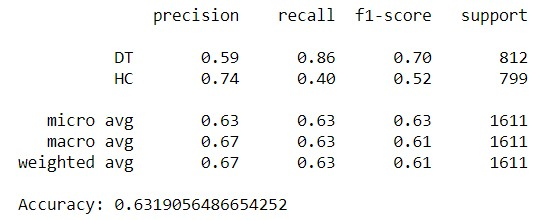
\includegraphics[width=\linewidth]{images/first_attempt_results.jpg}
  \caption{Results of first attempt of SVM with standard parameters}
  \label{fig:first_results}
\end{figure}

\section{K-fold Cross Validation}
After first results with SVM, to improve the performance of the model I used a K-fold Cross validation. In this method the training set is randomly partitioned into k equal sized subsamples. Each subsample will be used once as validation set, and the remaining portion as trianing set. The cross validation process is then repeated k times.\\
For this assignment I chose a 3 fold cross validation and as possible values to be evaluated:

\begin{itemize}
    \item C\_values = [ 0.1, 1, 10, 100, 1000 ]  
    \item gamma\_values = [ 1, 0.1, 0.01, 0.001, 0.0001 ]
\end{itemize}

\noindent After this i plotted the learning curve for the cross validation. This is shown in Figure \ref{fig:learning_curve}.

\begin{figure}[ht]
  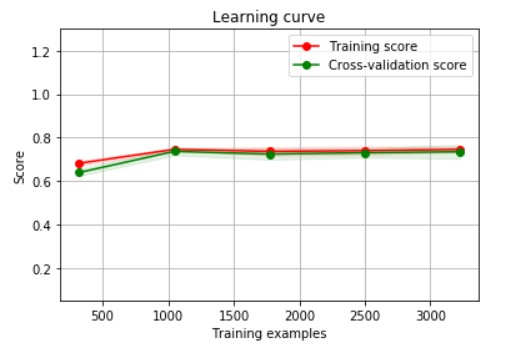
\includegraphics[width=\linewidth]{images/learning_curve.jpg}
  \caption{Learning curve of the k-fold cross validation}
  \label{fig:learning_curve}
\end{figure}

\section{Final Results}
After the cross validation the best parameters used are:

\begin{itemize}
    \item C = 1000  
    \item gamma = 1
\end{itemize}

\noindet I used this parameter to train once again the SVM on the training set and testing it on the test dataset. Results can be found in Figure \ref{fig:best_results}.\\
It's possible to see an improvement on the results from the first attempt (0.6319) to the final one(0.7865). It also possible to see that results are above the minimum value of accuracy (0.50403).

\begin{figure}[ht]
  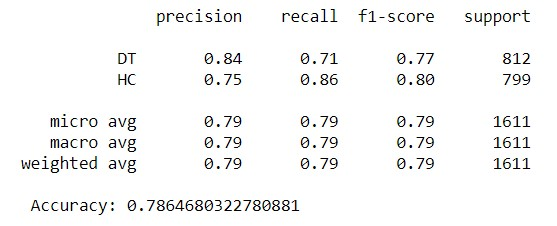
\includegraphics[width=\linewidth]{images/after_cv_results.jpg}
  \caption{Results with best parameters retrieved from cross validation}
  \label{fig:best_results}
\end{figure}

\end{document}
